\documentclass[xcolor=pdftex,dvipsnames,table,mathserif,aspectratio=169]{beamer}
\usetheme{metropolis}
%\usepackage{times}

\usepackage[english]{babel}
%\usepackage[table]{xcolor}
\usepackage{pgf,pgfarrows,pgfnodes,pgfautomata,pgfheaps}
\usepackage{amsmath,amssymb,setspace,outline}
\usepackage[latin1]{inputenc}
\usepackage[T1]{fontenc}
\usepackage{relsize}

\newcommand{\abs}[1]{\lvert#1\rvert}
\newcommand{\norm}[1]{\lVert#1\rVert}

%\usepackage{transparent}
\DeclareMathSizes{10}{10}{6}{6} 


\title [Single-agent dynamic optimization models]{Single-agent dynamic optimization models}
\author{C.Conlon - help from M. Shum and Paul Scott}
\institute{Grad IO }
\date{}
\setbeamercolor{figure}{bg=white}

\begin{document}
\title{MPEC notes}
\author{Chris Conlon\\
 thanks to Che-Lin Su}
\institute{Grad IO}
\date{\today}
\footnotesize
\frame{\titlepage}

\frame{\frametitle{Extremum Estimators}
Often faced with extremum estimator problems in econometrics (ML, GMM, MD, etc.)  that look like:
\begin{align*}
\hat{\theta} = \arg \max_{\theta} Q_n(\theta), \quad  \theta \in \Theta
\end{align*}
Many economic problems contain constraints, such as: market clearing (supply equals demand), consumer's consume their entire budget set, or firm's first order conditions are satisfied.  A natural way to represent these problems is as constrained optimization.
}

\begin{frame}{Constrained Problems}
\begin{block}{MPEC}
\begin{align*}
\hat{\theta} = \arg \max_{\theta,P} Q_n(\theta,P), \quad  \mbox{ s .t. } \quad \Psi(P,\theta) =0,  \quad \theta \in \Theta
\end{align*} 
\end{block}
\pause
\begin{block}{Fixed Point / Implicit Solution}
In much of the literature the tradition has been to express the solutions $\Psi(P,\theta) =0$ implicitly as $P(\theta)$:
\begin{align*}
\hat{\theta} = \arg \max_{\theta} Q_n(\theta,P(\theta)),  \quad \theta \in \Theta
\end{align*}
\end{block}
\end{frame}

\begin{frame}{NFXP vs MPEC}
Probably you were taught some things that weren't quite right
\begin{itemize}
\item Fewer parameters $\rightarrow$ easier problems to solve!
\item Reformulate problems with fixed points or implicit solutions to \alert{concentrate out} parameters.
\item But sometimes this makes the problem more complicated (saddle points, complicated Hessians, etc.)
\end{itemize}
MPEC says do the opposite:
\begin{itemize}
\item Add lots of parameters
\item But add them with simple constraints (linear or quadratic).
\item Idea: Make the Hessian as close to constant, block diagonal, sparse, etc. as possible.
\end{itemize}
Mostly this is in response to change in technology: nonlinear solvers supporting large sparse Hessians.
\end{frame}



\begin{frame}{Rust Problem}
\footnotesize
\begin{itemize}
\item Bus repairman sees mileage $x_t$ at time $t$ since last overhaul
\item Repairman chooses between overhaul and normal maintenance
\begin{align*}
u(x_t, d_t, \alert{\theta^c}, \alert{RC}) =
\begin{cases} -c(x_t,\alert{\theta^c}) \quad &\mbox{if} \quad d_t=0\\
-(\alert{RC} + c(0,\alert{\theta^c}) \quad) &\mbox{if} \quad d_t =1\\
\end{cases}
\end{align*}
\item Repairman solves DP:
\begin{align*}
V_{\alert{\theta}} (x_t) = \sum_{f_t,f_{t+1},\ldots} E \left\{  \sum_{j=t}^{\infty} \beta^{j-t}   [u(x_j,f_j,\alert{\theta}) + \varepsilon_{j}(f_j)]| x_t \right\}
\end{align*}
\end{itemize}
\begin{itemize}
%\item Observe mileage $x_t$ and decision $d_t$ but not cost.
%\item Assumes extreme value distribution for $\varepsilon_t(d_t)$
\item Structural parameters to be estimated $\alert{\theta = (\theta^c, RC, \theta^p)}$.
\item Coefficients of cost function $c(x,\alert{\theta^c}) = \theta^c_1 x + \theta^c_2 x^2$
\item Transition probabilities in mileages $p(x_{t+1} | x_t, d_t, \alert{\theta^p})$
\end{itemize}
\end{frame}


\begin{frame}{Rust Problem}
\begin{itemize}
\item Data: time series $(x_t,d_t)_{t=1}^T$
\item Likelihood function
\begin{align*}
\mathcal{L}(\theta) &= \prod_{t=2}^T P(d_t | x_t, \alert{\theta^c}, \alert{RC}) p(x_t | x_{t-1}, d_{t-1},\alert{\theta^p})\\
\mbox{ with }  P(d | x, \alert{\theta^c}, \alert{RC}) &= \frac{\exp[u(x,d,\alert{\theta^c},\alert{RC}) + \beta \textcolor{blue}{EV}_{\alert{\theta}}(x,d)}
{\sum_{d' \in \{0,1\}} \exp[u(x,d',\alert{\theta^c},\alert{RC}) + \beta \textcolor{blue}{EV}_{\alert{\theta}}(x',d)}\\
\textcolor{blue}{EV}_{\alert{\theta}}(x,d) &= T_{\alert{\theta}}(\textcolor{blue}{EV}_{\alert{\theta}})(x,d)\\
\end{align*}
\vspace{-1cm}
\begin{align*}
\equiv \int_{x'=0}^{\infty} &\log \left[ \sum_{d' \in \{0,1\}} \exp[u(x,d',\alert{\theta^c},\alert{RC}) + \beta \textcolor{blue}{EV}_{\alert{\theta}}(x',d)]  \right] p(dx' | x,d,\alert{\theta^p}) 
\end{align*}
\end{itemize}
\end{frame}


\begin{frame}{Rust Problem}
\begin{itemize}
\item Outer Loop: Solve Likelihood
\begin{align*}
\max_{\alert{\theta} \geq 0} \mathcal{L}(\theta) &= \prod_{t=2}^T P(d_t | x_t, \alert{\theta^c}, \alert{RC}) p(x_t | x_{t-1}, d_{t-1},\alert{\theta^p})\\
\end{align*}
\item Convergence test: $\norm{\nabla_{\theta} \mathcal{L}(\alert{\theta})} \leq \alert{\epsilon_{out}}$
\item Inner Loop: Compute expected value function $ \textcolor{blue}{EV}_{\alert{\theta}}$ for a given $\alert{\theta}$
\item $ \textcolor{blue}{EV}_{\alert{\theta}}$ is the implicit expected value function defined by the Bellman equation or the fixed point function
\begin{align*}
 \textcolor{blue}{EV}_{\alert{\theta}} = T_{\alert{\theta}}( \textcolor{blue}{EV}_{\alert{\theta}})
\end{align*}
\item Convergence test: $\norm{ \textcolor{blue}{EV}^{(k+1)}_{\alert{\theta}} - \textcolor{blue}{EV}^{(k)}_{\alert{\theta}} } \leq \alert{\epsilon_{in}}$
\item Start with contraction iterations and polish with Newton Steps
\end{itemize}
\end{frame}

\begin{frame}{NFXP Concerns}
\begin{itemize}
\item Inner-loop error propagates into outer-loop function and derivatives
\item NFXP needs to solve inner-loop exactly each stage of parameter search
\begin{itemize}
\item to accurately compute the search direction for the outer loop
\item to accurately evaluate derivatives for the outer loop
\item for outer loop to converge!
\end{itemize}
\item Stopping rules: choosing inner-loop and outer-loop tolerance
\begin{itemize}
\item inner loop can be slow: contraction mapping is linearly convergent
\item tempting to loosen inner loop tolerance $\alert{\epsilon_{in}}$ (such as $1e-6$ or larger!).
\item Outer loop may not converge with loose inner loop tolerance.
\begin{itemize}
\item check solver output message
\item tempting to loosen outer loop tolerance $\alert{\epsilon_{out}}$ to promote convergence ($1\text{e-}3$ or larger!).
\end{itemize}
\end{itemize}
\end{itemize}
\end{frame}

\begin{frame}{Convergence Properties (Su and Judd)}
\begin{itemize}
\item $\mathcal{L}(\textcolor{blue}{EV}(\alert{\theta},\alert{\epsilon_{in}} ), \alert{\theta} )$ the programmed outer loop objective function
\item $L$: the Lipschitz constant (like modulus) of inner-loop contraction mapping
\item Analytic derivatives $\nabla_{\theta} \mathcal{L}(\textcolor{blue}{EV}(\alert{\theta},\alert{\epsilon_{in}} ), \alert{\theta} )$ is provided: $\alert{\epsilon_{out}} = O(\frac{L}{1-L} \alert{\epsilon_{in}})$
\item Finite-difference derivatives are used: $\alert{\epsilon_{out}} = O ( \sqrt{\frac{L}{1-L}} \alert{\epsilon_{in}} )$ 
\end{itemize}
\end{frame}

\begin{frame}{MPEC Alternative (Su and Judd))}
\begin{itemize}
\item Form the augmented likelihood function for data $X = (x_t, d_t)_{t=1}^T$
\begin{align*}
\mathcal{L}(\textcolor{blue}{EV}, \alert{\theta}; X) &= \prod_{t=2}^T P(d_t | x_t, \alert{\theta^c}, \alert{RC}) p(x_t | x_{t-1}, d_{t-1},\alert{\theta^p})\\
\mbox{ with }  P(d | x, \alert{\theta^c}, \alert{RC}) &= \frac{\exp[u(x,d,\alert{\theta^c},\alert{RC}) + \beta \textcolor{blue}{EV}(x,d)}
{\sum_{d' \in \{0,1\}} \exp[u(x,d',\alert{\theta^c},\alert{RC}) + \beta \textcolor{blue}{EV}(x',d)}\\
\end{align*}
\item Rationality and Bellman equation imposes a relationship between $\alert{\theta}$ and $\textcolor{blue}{EV}$
\begin{align*}
\textcolor{blue}{EV} = T(\textcolor{blue}{EV},\alert{\theta})
\end{align*}
\item Solve constrained optimization problem
\begin{align*}
\max_{(\alert{\theta},\textcolor{blue}{EV})} \mathcal{L}(\textcolor{blue}{EV}, \alert{\theta}; X)\\
\mbox{ subject to }  \textcolor{blue}{EV} = T(\textcolor{blue}{EV},\alert{\theta})
\end{align*}
\end{itemize}
\end{frame}


\begin{frame}{MPEC Alternative$^2$}
The previous approach solves the problem ``on the grid''.
\begin{itemize}
\item $x_t$ takes on discrete values.
\item We only evaluate $EV(x_t,i_t)$ at values on the grid.
\item We don't evaluate $EV(x_t,i_t)$ and values between $[x_s,x_{s+1}]$.
\end{itemize}
If we did we would have to \alert{interpolate}.
\begin{itemize}
\item Macroeconomists tend to use \alert{cubic splines}
\item Could use global orthogonal polynomials $EV(x) \approx a_0 + a_1 b_1(x)+ a_2 b_2(x) + \ldots$
\begin{itemize}
\item Advantage is that solving polynomial equation for $\textcolor{blue}{EV} = T(\textcolor{blue}{EV},\alert{\theta})$ is pretty easy.
\item Can easily switch to continuous state space without any additional complications:  $f(x_{t+1} | x_{t})$ must also be continuous.
\end{itemize}
\end{itemize}
\end{frame}

\frame{\frametitle{Results}

\begin{figure}[htbp]
\begin{center}
\color{transparent}
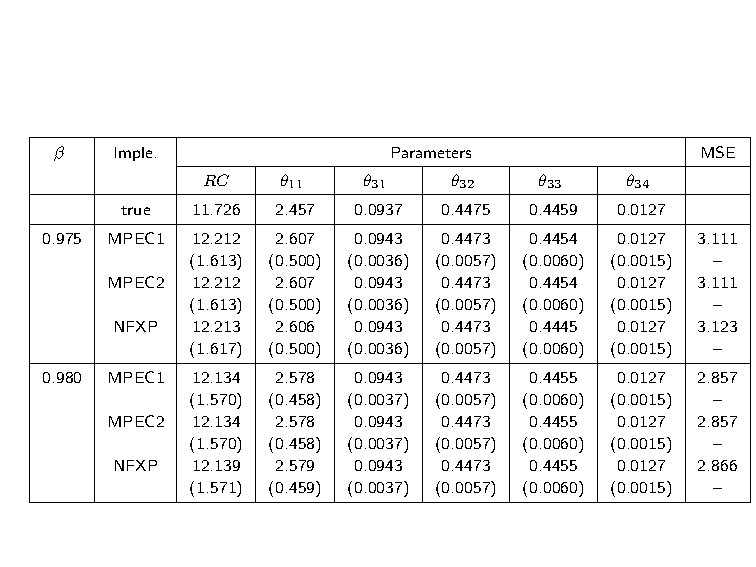
\includegraphics[width=4.5in]{resources/su1.pdf}
\end{center}
\end{figure}
}

\frame{\frametitle{Results}
\begin{figure}[htbp]
\begin{center}
\color{transparent}
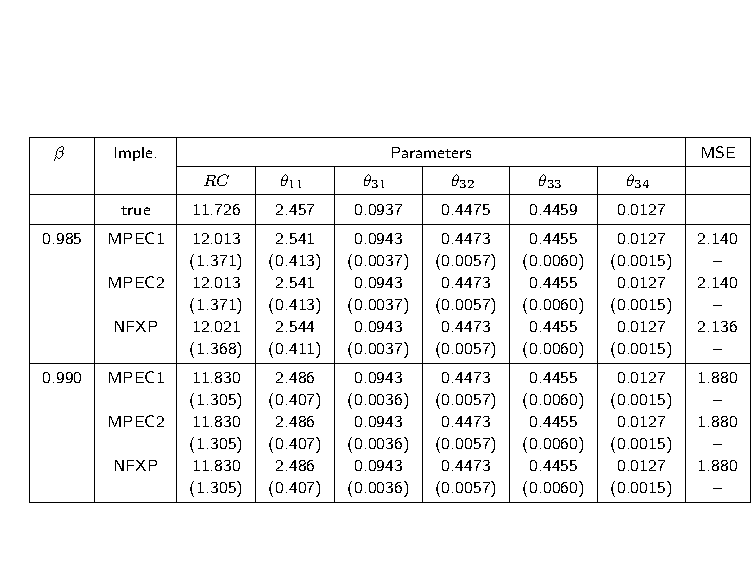
\includegraphics[width=4.5in]{resources/su2.pdf}
\label{default}
\end{center}
\end{figure}
}
\frame{\frametitle{Results}
\begin{figure}[htbp]
\begin{center}
\color{transparent}
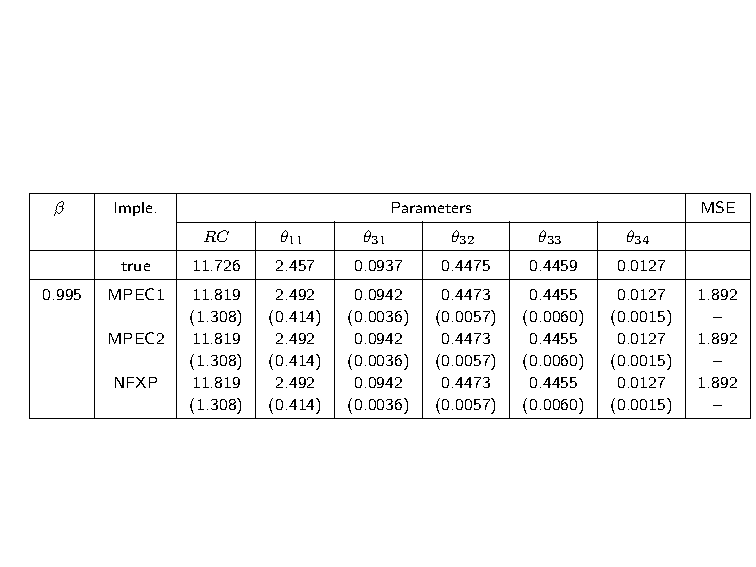
\includegraphics[width=4.5in]{resources/su3.pdf}
\label{default}
\end{center}
\end{figure}
}
\frame{\frametitle{Results}
\begin{figure}[htbp]
\begin{center}
\color{transparent}
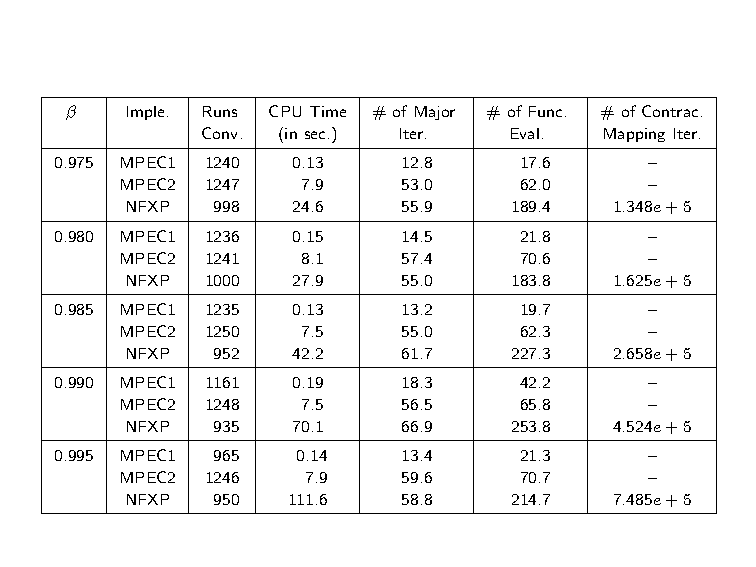
\includegraphics[width=4.5in]{resources/su4.pdf}
\label{default}
\end{center}
\end{figure}
}
\frame{\frametitle{Results}
\begin{figure}[htbp]
\begin{center}
\color{transparent}
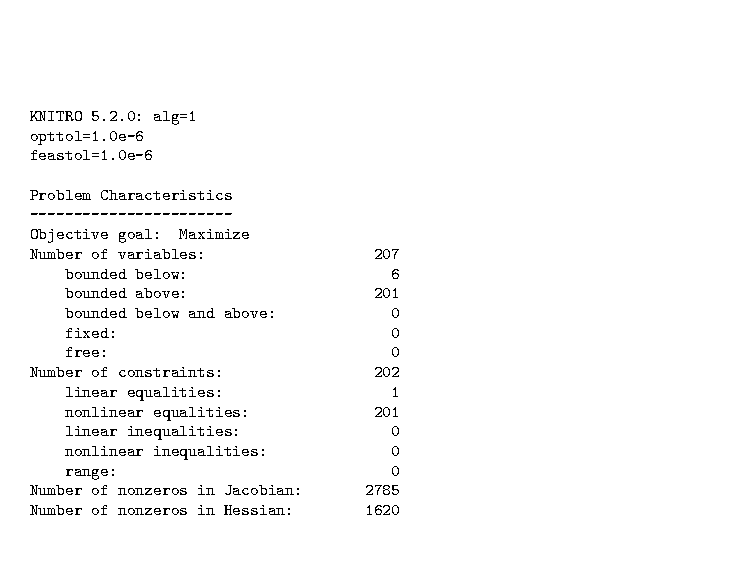
\includegraphics[width=2.5in]{resources/su5.pdf}
\label{default}
\end{center}
\end{figure}
}
\frame{\frametitle{Results}
\begin{figure}[htbp]
\begin{center}
\color{transparent}
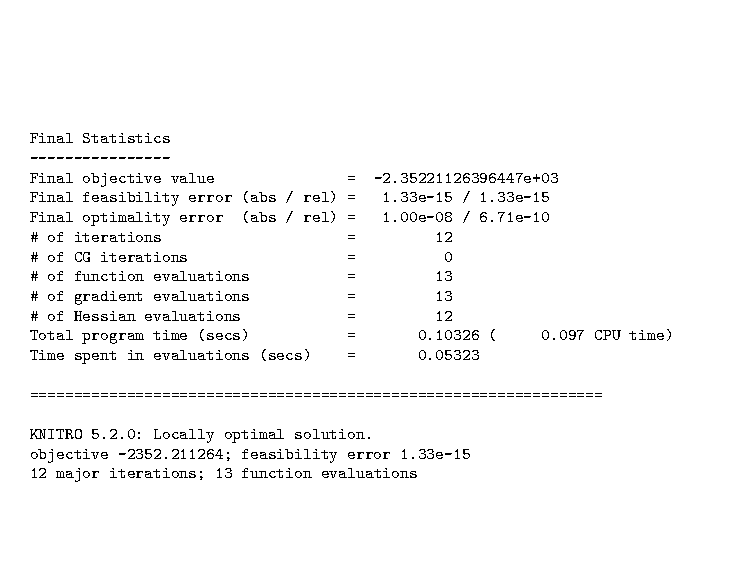
\includegraphics[width=4.5in]{resources/su6.pdf}
\label{default}
\end{center}
\end{figure}
}

\frame{\frametitle{BLP Demand Example}
\begin{exampleblock}{BLP 1995}
The estimator solves the following mathematical program:
\begin{align*}
\min_{\alert{\theta_2}} & g(\xi(\alert{\theta_2}))' W g(\xi(\alert{\theta_2})) \quad \mbox{ s.t. } \\
g(\xi(\alert{\theta_2})) &= \frac{1}{N} \sum_{\forall j,t} \xi_{jt} (\alert{\theta_2}) ' z_{jt} \\
\xi_{jt}(\alert{\theta_2}) &= \delta_j(\alert{\theta_2}) - x_{jt} \beta - \alpha p_{jt} \\
s_{jt}(\delta(\alert{\theta_2}),\alert{\theta_2}) &= \int \frac{\exp[\delta_j(\alert{\theta_2})+ \mu_{ij}]}{1+\sum_k \exp[\delta_j(\alert{\theta_2})+ \mu_{ik}]} f(\mu | \alert{\theta_2})\\
\log(S_{jt})  &= \log(s_{jt}(\delta(\alert{\theta_2}),\alert{\theta_2})) \quad \forall j,t
\end{align*}
\end{exampleblock}
}

\frame{\frametitle{BLP Algorithm}
The estimation algorithm is generally as follows:
\begin{enumerate}
\item Guess a value of nonlinear parameters $\alert{\theta_2}$
\item Compute $s_{jt}(\delta,\alert{\theta_2})$ via integration
\item Iterate on $\delta_{jt}^{h+1}  = \delta_{jt}^h +  \log(S_{jt}) - \log(s_{jt}(\delta^{h},\alert{\theta_2}))$ to find the $\delta$ that satisfies the share equation
\item IV Regression $\delta$ on observable $X$ and instruments $Z$ to get residual $\xi$.
\item Use $\xi$ to construct $g(\xi(\alert{\theta_2}))$.
\item Possibly construct other errors/instruments from supply side.
\item Construct GMM Objective
\end{enumerate}
The idea is that $\delta(\alert{\theta_2})$ is an implicit function of the nonlinear parameters $\alert{\theta_2}$. And for each guess we find that implicit solution for reduce the parameter space of the problem. But the Jacobian: $\frac{\partial \boldsymbol{\xi_t}}{\partial \theta_2}(\theta_2) = -{\left[\frac{\partial \boldsymbol{s}_t}{\partial \boldsymbol{\delta_t}}(\theta_2)\right]^{-1} \left[\frac{\partial \boldsymbol{s}_t}{\partial \theta_2}(\theta_2)\right]} $ is complicated to compute.
}



\frame{\frametitle{Dube Fox Su 2012}
\begin{exampleblock}{BLP-MPEC}
The estimator solves the following mathematical program:
\begin{align*}
\label{blpmpec}
\min_{\alert{\sigma,\alpha,\beta, \xi}}  & g(\alert{\xi})' W g(\alert{\xi}) \quad \mbox{ s.t. } \\
g(\alert{\xi}) &= \frac{1}{N} \sum_{\forall j,t} \alert{\xi_{jt}'} z_{jt} \\
s_{jt}(\alert{\sigma,\alpha,\beta, \xi}) &=  \sum_i w_i \frac{\exp[x_{jt} \alert{\beta} + \alert{\xi_{jt}} - \alert{\alpha} p_{jt} + \sum_l \nu_{il} x_{jt}^l \alert{\sigma_l} ] }
{1+ \sum_k \exp[x_{kt} \alert{\beta} + \alert{\xi_{kt}} - \alert{\alpha} p_{kt} + \sum_l \nu_{il} x_{kt}^l \alert{\sigma_l} ]} \\
\log(S_{jt})  &= \log s_{jt}(\alert{\sigma,\alpha,\beta, \xi}) \quad \forall j,t
\end{align*}
\end{exampleblock}
\begin{itemize}
\item Expand the parameter space of the nonlinear search to include $\alert{\alpha,\beta,\xi}$
\item Don't have to solve for $\xi$ except at the end.
\item No implicit functions of $\theta_2$ and $\left[\frac{\partial \boldsymbol{s}_t}{\partial \sigma}(\alert{\sigma,\alpha,\beta, \xi})\right]$ is straightforward (no matrix inverse!).
\item Sparsity!
\end{itemize}
}




\frame{\frametitle{Nevo Results}
\begin{center}
\rowcolors[]{1}{RoyalBlue!5}{RoyalBlue!15} 
\begin{tabular}{lrrrr}
& Nevo & BLP-MPEC & EL\\
Price& -28.189  & -62.726  & -61.433  \\
$\sigma_{p}$ &0.330 & 0.558 & 0.524\\
$\sigma_{const}$ &2.453 &3.313 & 3.143\\
$\sigma_{sugar} $& 0.016&-0.006 & 0\\
$\sigma_{mushy} $&0.244 &0.093&0.085\\
$\pi_{p,inc}$ &15.894  &588.206 & 564.262\\
$\pi_{p,inc2}$ &-1.200  &-30.185 &-28.930 \\
$\pi_{p,kid}$ &2.634 &11.058 &   11.700\\
$\pi_{c,inc}$ &5.482 & 2.29084&2.246\\
$\pi_{c,age} $& 0.2037&1.284 & 1.37873 \\
GMM &29.3611 &4.564 & \\
EL & & &-17422  \\
Time & 28 s & 12s & 19s  \\
\end{tabular}
\end{center}
}



\end{document}


